\documentclass[]{article}
\usepackage{lmodern}
\usepackage{amssymb,amsmath}
\usepackage{ifxetex,ifluatex}
\usepackage{fixltx2e} % provides \textsubscript
\ifnum 0\ifxetex 1\fi\ifluatex 1\fi=0 % if pdftex
  \usepackage[T1]{fontenc}
  \usepackage[utf8]{inputenc}
\else % if luatex or xelatex
  \ifxetex
    \usepackage{mathspec}
  \else
    \usepackage{fontspec}
  \fi
  \defaultfontfeatures{Ligatures=TeX,Scale=MatchLowercase}
\fi
% use upquote if available, for straight quotes in verbatim environments
\IfFileExists{upquote.sty}{\usepackage{upquote}}{}
% use microtype if available
\IfFileExists{microtype.sty}{%
\usepackage{microtype}
\UseMicrotypeSet[protrusion]{basicmath} % disable protrusion for tt fonts
}{}
\usepackage[unicode=true]{hyperref}
\hypersetup{
            pdfborder={0 0 0},
            breaklinks=true}
\urlstyle{same}  % don't use monospace font for urls
\usepackage{graphicx,grffile}
\makeatletter
\def\maxwidth{\ifdim\Gin@nat@width>\linewidth\linewidth\else\Gin@nat@width\fi}
\def\maxheight{\ifdim\Gin@nat@height>\textheight\textheight\else\Gin@nat@height\fi}
\makeatother
% Scale images if necessary, so that they will not overflow the page
% margins by default, and it is still possible to overwrite the defaults
% using explicit options in \includegraphics[width, height, ...]{}
\setkeys{Gin}{width=\maxwidth,height=\maxheight,keepaspectratio}
\IfFileExists{parskip.sty}{%
\usepackage{parskip}
}{% else
\setlength{\parindent}{0pt}
\setlength{\parskip}{6pt plus 2pt minus 1pt}
}
\setlength{\emergencystretch}{3em}  % prevent overfull lines
\providecommand{\tightlist}{%
  \setlength{\itemsep}{0pt}\setlength{\parskip}{0pt}}
\setcounter{secnumdepth}{0}
% Redefines (sub)paragraphs to behave more like sections
\ifx\paragraph\undefined\else
\let\oldparagraph\paragraph
\renewcommand{\paragraph}[1]{\oldparagraph{#1}\mbox{}}
\fi
\ifx\subparagraph\undefined\else
\let\oldsubparagraph\subparagraph
\renewcommand{\subparagraph}[1]{\oldsubparagraph{#1}\mbox{}}
\fi

% set default figure placement to htbp
\makeatletter
\def\fps@figure{htbp}
\makeatother


\date{}

\begin{document}

\begin{quote}
\textbf{EPIFISIOLISI}
\end{quote}

\textbf{Definizione:} in conseguenza di un cedimento della zona di
coniugazione tra epifisi prossimale e collo femorale, l'epifisi si
distacca e scivola in basso e indietro mettendosi in rapporto con il
lato mediale del collo femorale. L'anca subisce un varismo e questa
condizione predispone ad un'artosi secondaria precoce.

\begin{quote}
\textbf{EPIDEMIOLOGIA e PATOGENESI}
\end{quote}

Incidenza 2/10 \^{}5, maschi:femmine= 2,5 : 1, età maschi 10-14 anni ,
età femmine 10-16 anni, bilaterale nel 25-50\% dei casi

\begin{itemize}
\item
  \textbf{ipotesi meccanica}: l'obesità o il sovrappeso (spesso presenti
  nei soggetti affetti), un'eccessiva richiesta funzionale, un ginocchio
  valgo, un piede piatto sono tutte condizioni che portano
  all'applicazione di forze a livello del collo femorale che ne inducono
  un gioco di leve in grado di dissecare l'epifisi in accrescimento
\item
  \textbf{ipotesi distrofico-metabolica}: in soggetti che hanno una
  lassità legamentosa costitutiva o genetica presentano epifisiolisi in
  conseguenza dei maggiori movimenti permessi all'articolazione lassa
  dell'anca in accrescimento.
\end{itemize}

\begin{quote}
\textbf{CLINICA}
\end{quote}

\begin{enumerate}
\def\labelenumi{\arabic{enumi}.}
\item
  \textbf{Quadro di epifisiolisi cronica (85\% dei casi)}: le
  alterazioni si instaurano gradualmente nel corso di settimane durante
  le quali il giovane paziente accusa dolore localizzato all'inguine o
  alla coscia/ginocchio mediale che recede con il riposo, c'è
  limitazione alla intrarotazione e all'abduzione che nelle fasi più
  avanzate saranno compromesse completamente. Ne risulta una tipica
  andatura con zoppia. Alla radiografia si nota un'aumento dello
  spessore della linea di congiunzione cervico- epifisaria i cui margini
  sono irregolari e la struttura dell'osso sottostante presenta
  un'alternarsi di zone opache e trasparenti indicative del fenomeno ad
  andamento cronico (sono espressione di precedenti episodi di micro
  epifisiolisi).Negli stadi più avanzati il collo femorale è scoperto
  nella sua porzione supero-mediale mentre l'epifisi prossimale è a
  contatto con la zona inferiore e mediale del collo.Il trattamento può
  essere conservativo nelle fasi iniziali e consiste nell'applicazione
  di viti e chiodi transtrocanteriche che, dopo aver raggiunto una
  riduzione dell'epifisi sul collo femorale, fissano le strutture
  diastatizzate e ne permettono una stabilità morfologica e funzionale
  (vedi immagine).
\item
  \textbf{Quadro di epifisolisi acuta o epifisiolisi acuta su
  cronica(15\% dei casi)}: la presetnazione è uguale alle fratture
  cervico-epifisiaria e comprende un dolore acuto all'inguine o alla
  coscia mediale associato ad una grave impotenza funzionale e alla
  presentazione dell'arto come accorciato addotto e extraruotato. Il
  trattamento deve essere precoce e si compone ancora una volta di
  riduzione e fissazione dell'epifisi al collo del femore con viti e
  chiodi.
\end{enumerate}

\begin{quote}
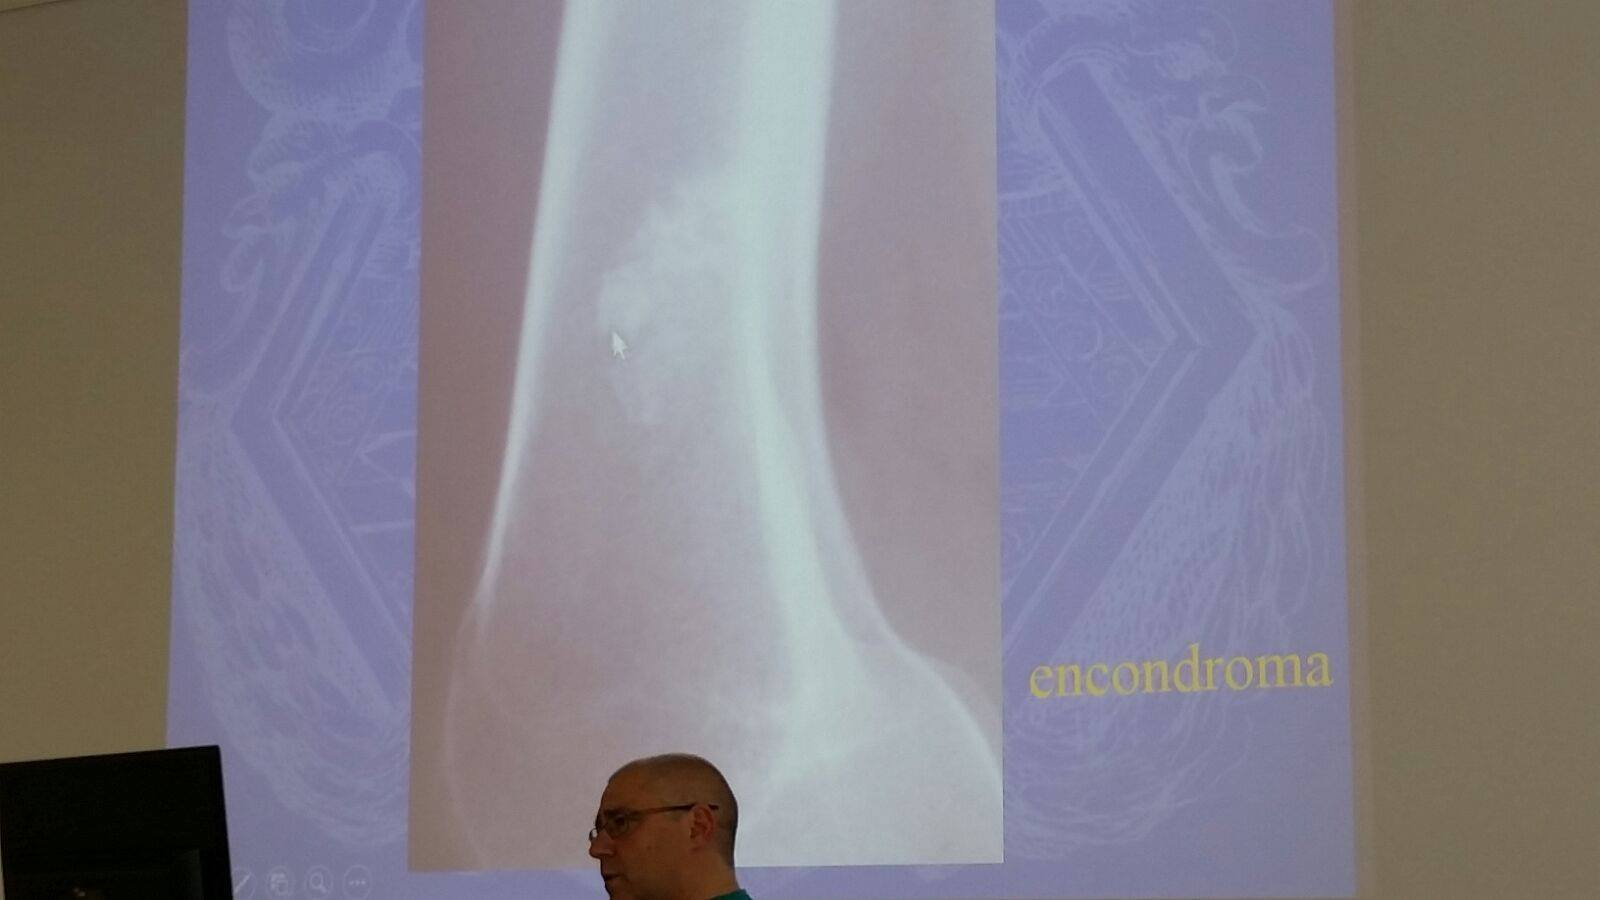
\includegraphics[width=3.07639in,height=2.01806in]{media/image1.jpeg}

\textbf{OSTEOCONDROSI}
\end{quote}

\textbf{Definizione:} è un insieme di patologie caratterizzato dalla
contemporanea presenza di necrosi ischemica dell'osso, di una
degenerazione della cartilagine limitrofa che esitano in microfratture
ripetute che possono localizzarsi nelle seguenti strutture:

\begin{itemize}
\item
  nucleo epifisiario: epifisi prossimale del femore (malattia di
  Perthes), epifisi metatarsale (generalmente testa del secondo)
\item
  osso breve : scafoide tarsico;
\item
  superficie convessa di una articolazione cartilaginea ( osteocondrite
  dissecante): condilo femorale mediale, testa del femore, condilo
  omerale, troclea astragalica.
\end{itemize}

\textbf{PATOGENESI}

Generalmente colpisce soggetti giovani in accrescimento, come
l'epifisiolisi. La zona anatomica interessata dalla necrsosi ischemica è
una zona la cui vascolarizzazione è esposta a delle limitazioni
anatomiche in quanto l'osso in accrescimento è circondato da cartilagine
jalina perforata da microvasi. Qualunque alterazione della cartilagine
(a base genetica, familiare o aquisita da traumi ecc) può portare alla
obliterazione di questi vasi e questo innesca un circolo vizioso
vascolare-meccanico che mantiene il danno cartilagineo e osseo e lo
amplifica fino a coinvolgere l'intera zona ed esita in un distacco
patologico.

\begin{quote}
\textbf{PATOLOGIE}
\end{quote}

\textbf{Malattia di Perthes.} incidenza 1,5/10\^{}5 aa, maschi.femmine=
5:1, età 3-14, 90\% monolaterale.

Come ogni affezione dolorosa di questa zona il dolore è riferito
all'inguine o alla faccia interna della coscia, c'è limitazione
funzionale in particolare dei movimenti abduttori e rotativi, la marcia
presenta zoppia.

Radiograficamente si distinguono 4 gradi di gravità che vedono un
progressivo peggioramento del capo articolare interessato il quale
inizialmente presenta una semplice irregolarità del contorno e della
trabecolatura ossea , quando inizia a comparire la necrosi sia ha un
aumento dell'opacità e uno schiacciamento del profilo del nucleo
epifisario, ancora dopo insorgono fenomeni di rimaneggiamento osseo e di
riparazione che portano ad un profilo totalmente irregolare di entrambi
i capi articolari, configurandosi dunque una coxartrosi precoce.

Terapia: nelle fasi iniziali ci si può permettere l'applicazione di
misure conservative quali apparecchi gessati o tutori utilizzati per
lunghi periodi che, associati a un controllo del peso corporeo,
stabilizzano la situazione e ne prevengono un' ulteriore involuzione.
Nei gradi più avanzati il trattamento è chirurgico e si eseguono
interventi volti a migliorare la congruenza fra acetabolo e testa del
femore o a mettere in scarico i punti di contatto articolari con
un'osteotomia e una rotazione di 180° del collo femorale con l'obiettivo
di limitare la necrosi epifisiaria.

\textbf{Apofisiolisi di Osgood-Schalatter} (vale anche per apofisi
calcaneale e apofisi della tuberosità ischiatica) : si tratta di un
distacco e una degenerazione della cartilagine nel punto di inserzione
dei tendini del muscolo quadricipite femorale nella tibia. Durante
l'accrescimento infatti coesistono due situazioni disarmoniche: le masse
muscolari si accrescono velocemente e acquisiscono sempre più potenza
mentre la cartilagine su cui esercitano trazioni i loro tendini
d'inserzione è ancora in via di sviluppo e consolidazione,
sostazialmente incapace di sopportare una trazione violenta. Questi
distacchi parcellari sono classificabili come fratture da fatica e
guariscono con il riposo. La forte sintomatologia dolorosa locale,
esacerbata dall'azione del muscolo e migliorata dal riposo, trae
beneficio da tecniche fisiche locamente applicate, come vedremo nelle
lezioni di fisiatria.

\begin{quote}
\textbf{Osteocondrosi di metatarso intermedio e di scafoide tarsico}:
sono cause di dolore al piede in età giovanile, specialmente nei maschi,
specialmente in concomitanza di attività fisica intensa.
\end{quote}

Le radiografie hanno caratteristiche anatomo-patologiche simili a quelle
identificate per la malattia di Perthes e il trattamento d'elezione è lo
scarico funzionale della regione. Solo in rari casi dove l'anatomia
delle ossa e delle articolazioni è molto compromessa e la sintomatologia
dolorosa non regredisce e dunque si accede alla chirurgia che riassesta
l'assetto articolare con osteotomie e/o artrodesi.

\textbf{Osteocondrosi dissecante}: come prima accennato sono patologie
delle superfici convesse delle articolazioni dotate di cartilagine
jalina e sottoposte a traumi tangenziali ripetuti (attività sportive,
cadute e tutte le altre attività potenzialmente traumatizzanti svolte
dai bambini).

Il segmento interessato dalla patologia ischemico-necrotizzante fa si
che porzioni di superficie articolare si distacchino e migrino
all'interno della cavità articolare, nel tempo si accrescono perchè
nutriti per diffusione dal liquido sinoviale e danno segno di se con
dolore e tumefazione articolare. La terapia dipende dalla gravità del
quadro clinico e, quando necessaria, la chirurgia è impiegata per
fissare l'elemento vagante con viti, dopo aver cruentato il letto
accogliente sul lato articolare per fare in modo che si crei un callo
osseo in grado di ristabilire la continuità con il segmento stesso.

\begin{quote}
\textbf{METATARSALGIE}
\end{quote}

METATARSALGIA (qualunque dolore che interessa il metatarso, cioè la
parte anteriore del piede, sia plantare che dorsale).

Seconda causa di sofferenza (dopo mal di testa) del corpo umano.

Metatarso è una parte del piede costituita dalle ossa metatarsali (1°,
2°, 3°, 4°, 5° osso metatarsale).

\emph{Classificazione:}

\textbf{METATARSALGIE NON MECCANICHE}

\begin{itemize}
\item
  osteocondrosi
\item
  artrosi
\item
  infezioni
\item
  neoplasie
\item
  malattie vascolari
\item
  malattie neurologiche (sindrome tunnel tarsale)
\item
  malattie metaboliche (gotta, diabete)
\item
  malattie dermatologiche (micosi, psoriasi)
\end{itemize}

\begin{quote}
\textbf{METATARSALGIE MECCANICHE} (alterazioni della struttura)

\textbf{\emph{METATARSALGIE NON MECCANICHE}}
\end{quote}

ESITI DI OSTEOCONDROSI

Esempio necrosi seconda testa metatarsale da bambini, solitamente in
fase acuta non si fa diagnosi, il dolore si autolimita, ma la testa
invece di essere rotonda è schiacciata.

Nell'adulto tipico dolore nella fase di spinta (nella flessione dorsale
del piede).

Terapia: rimodellare la testa metatarsale, artroplastica (si tolgono gli
osteofiti e si cerca di dare un minimo di rotondità alla testa);
solitamente c'è un frammentino mobile a livello dorsale, che è quello
che crea dolore durante la flessione dorsale.

ARTRITE REUMATOIDE (O PSORIASICA) IN FASE ACUTA

Artrite reumatoide colpisce la membrana sinoviale, per cui interessa
soprattutto piede e mano che sono le strutture maggiormente
sinovializzate (non è infrequente che un'artrite reumatoide inizi con
una meta tarsalgia).

\begin{quote}
Quando il paziente è in piedi e le dita sono allargate e soprattutto non
toccano, senza deformità: iperplasia della membrana sinoviale, no perché
c'è liquido.
\end{quote}

INFEZIONI

Es causate da ferite da punta, o comunque infezioni croniche con il
tipico granuloma.

Trattamento: fere in modo che tutto il materiale necrotico e il pus esca
e soprattutto che la ferita non si chiuda in un tempo troppo breve (per
cui drenaggi) in modo che la ferita si spurghi e che gli antibiotici
possano agire.

NEOPLASIE

Es fibrosarcoma (tumore maligno)

Neuroma di Morton (tumore benigno): tumore (non si è capito se è un
fibroma, un neuro fibroma,..) che si sviluppa a livello plantare tra la
terza e quarta testa del nervo digitale comune, prima che si biforchi
nei due digitali propri. Il nervo digitale comune in questo modo viene
in contatto con il legamento intermetatarsale (tra le due teste) e
sfregando si crea un tipica sintomatologia che va dal dolore, al
bruciore, alla sensazione di scossa elettrica che interessa i margini
contrapposti del terzo e quarto dito.

Mulder test: si sente un click tattile a volte anche uditivo quando
manualmente stringiamo le teste metatarsali, perche il neuroma, come un
piccolo pallino schizza fuori e in più si riproduce la tipica
sintomatologia.

Anatomia patologica del neuroma è varia, forse è dovuto a un problema
meccanico, cioè una condizione di sovraccarico sui raggi esterni, come
in caso di alluce valgo (per insufficienza del 1°raggio c'è uno
spostamento del carico sui raggi esterni) e alluce rigido.

Non c'è modo di fare diagnosi (no ecografia, no risonanza)

La sintomatologia è indipendente dalla grandezza del neuroma.

Trattamento chirurgico: accesso dal di sopra (no dalla pianta), si
isolano il nervo digitale comune e nervi digitali propri, e si toglie il
neuroma, cioè si tolgono i nervi per cui si passa da una condizione di
ipersensibilità a una di ipo-anestesia dopo l'intervento (è stato
dimostrato poi che a distanza di anni la sensibilità torna perché le
terminazioni nervose tornano a innervare le zone).

SINDROME DEL TUNNEL TARSALE

Nervo tibiale posteriore e arteria tibiale posteriore passano dietro al
malleolo interno, nel canale del tarso (simile al canale del carpo). Per
cui se c'è una compressione del canale (esempio per una cisti),
compressione del nervo e quindi meta tarsalgia. Di fatto la sindrome del
tunnel tarsale non è mai ascrivibile, come anatomia patologica, alla
compressione del mediano al carpo (che si verifica perche le guaine dei
tendini si gonfiano, per una cisti, per esiti di frattura). In realtà
nella sindrome del tunnel tarsale non c'è una compressione, non c'è una
sproporzione tra contenente e contenuto come per il tunnel carpale, ma è
una sindrome da stiramento (come quando si ha un valgo di retro-piede,
eccesso di pronazione, quindi rotazione esterna del calcagno, tutte le
strutture interne vengono sottoposte ad una trazione eccessiva). Per cui
non bisogna trattare la sindrome del tunnel tarsale come quella del
tunnel carpale, perche avremmo un risultato negativo considerando che
non bisogna decomprimere ma raddrizzare il retro-piede.

Si può avere anche un intrappolamento, contusione, stiramento dei nervi
anteriori, es. nervo peroneo superficiale (solo sensitivo); in questo
caso si valuta il segno di Tinel. Intrappolamento si può verificare in
persone che dimagriscono rapidamente: il nervo all'uscita della fascia
rimane appunto intrappolato.

PATOLOGIE SOVRASEGMENTARIE

Ernia del disco con interessamento ad esempio solo del nervo sciatico
popliteo interno, per cui meta tarsalgia. Oppure lo sciatico popliteo
esterno, che passa a livello del collo prossimale del perone: una
qualunque patologia della sindesmosi (articolazione) tibia-perone
prossimale, come una cisti, può andare a comprimere il nervo per cui
dolore alla dorsale del piede.

ISCHEMIA

Ad esempio nei diabetici, nei fumatori forti, può provocare la classica
sindrome del dito blu, il sangue arriva poco e c'è stasi per cui
deossigenazione. Arteriografia.

IPOTROFIA DEL PANNICOLO ADIPOSO PLANTARE

Meta tarsalgia ``meccanica'', anche se non è sostenuta da cause
meccaniche, riduzione dello spessore del pannicolo adiposo. Pelle lassa.

CICATRICI PLANTARI

Meta tarsalgia non meccanica: ad esempio se qualche chirurgo ha tolto il
neuroma di Morton per via plantare, si crea una cicatrice nella zona di
carico con ipertrofia.

CHERATOMA PLANTARE

Tumore benigno, si crea nelle zone di sovraccarico; ipercheratosi, callo
con metaplasia. Asportazione chirurgica.

VERRUCHE PLANTARI E RAGADI PLANTARI (spaccamento della pelle).

\begin{quote}
\textbf{\emph{METATARSALGIE MECCANICHE }}
\end{quote}

Determinate da una alterazione della meccanica dell'avampiede per:

-pressione più elevata a livello di una testa metatarsale

-pressione normale applicata per un periodo di tempo maggiore ( come
nell'eccesso di pronazione / supinazione)

classificazione:

\begin{enumerate}
\def\labelenumi{\arabic{enumi}.}
\item
  sovraccarico globale dell'avampiede
\item
  distribuzione irregolare del carico metatarsale
\end{enumerate}

Sono caratterizzare tutte dal CALLO, perché sia che ci sia un aumento
del carico, quantitativo o temporale, la pelle rimane schiacciata, si
crea un'ischemia e reagisce aumentando lo spessore dello strato corneo,
per cui il callo è una reazione al sovraccarico. Per cui per togliere i
calli si deve intervenire chirurgicamente o con dei plantari per
riequilibrare la distribuzione del carico.

N.B.: NON E' ASSOLUTAMENTE VERO CHE IL PESO APPOGGIA SOLO SUL 1° E SUL
5° DITO, TUTTE LE TESTE METATARSALI DEVONO APPOGGIARE IN MODO UGUALE (SE
UNO HA UN ARCO TRASVERSO, CIOE' 1° E 5° E' PATOLOGIA; FISIOLOGICAMENTE
ESISTE SOLO L'ARCO LONGITUDINALE)

\begin{itemize}
\item
  \textbf{\emph{sovraccarico globale dell'avampiede}}: tutte le teste
  metatarsali soffrono. Cause:
\end{itemize}

\begin{itemize}
\item
  calzature con tacco eccessivo: per ogni cm in altezza del tacco il
  peso si sposta di una certa \% a livello della zona metatarsale (tacco
  fisiologico 3-4 cm).
\item
  piede equino rigido, per mancata dorsi-flessione del piede, trattabile
  con un allungamento del tendine di achille.
\item
  piede cavo, slivellamento tra avampiede e retro piede, con
  sovraccarico dell'avampiede e del tallone anteriore inteso come zona
  di appoggio anteriore metatarsale.
\end{itemize}

\begin{itemize}
\item
  \textbf{\emph{distribuzione irregolare del carico metatarsale}}:
\end{itemize}

\begin{enumerate}
\def\labelenumi{\alph{enumi}.}
\item
  \textbf{insufficienza del 1° raggio} (tra cui alluce valgo), che porta
  al sovraccarico dei raggi esterni. Alluce valgo: deviazione laterale
  1° dito sostenuto da un allargamento del ventaglio metatarsale
  (metatarso varo), aumento dell'angolo intermetatarsale (tra 1° e 2°
  metatarso); le cause sono numerose, ricordiamo:
\end{enumerate}

\begin{itemize}
\item
  cause biomeccaniche (più frequenti) come durante la gravidanza e dopo
  la menopausa;
\item
  predisposizione genetica (a seconda dell'anatomia abbiamo diversi tipi
  di piede, tutti normali: formula digitale: piede egizio -- primo dito
  più lungo del secondo,
\end{itemize}

\begin{quote}
piede greco -- primo dito più corto del secondo, piede quadrato -- primo
e secondo dito uguali;

formula metatarsale: index plus-minus - primo e secondo metatarsali sono
uguali, index minus -- primo metatarsale più corto del secondo, index
plus -- primo metatarsale più lungo del secondo);
\end{quote}

tra queste formule digitali e metatarsali la condizione sfavorevole per
la patogenesi dell'alluce valgo è l'associazione piede egizio + index
minus.

\begin{quote}
- pronazione del retro piede (es nel piede piatto).
\end{quote}

Tutte le altre, come i tacchi alti sono concause, no cause di alluce
valgo.

Quello che succede a livello del 1°raggio, può succedere anche a livello
del 4° e 5° raggio, con un allargamento dell'angolo tra quarto e quinto,
per cui c'è un allargamento del primo e del quinto con formazione
dell'avampiede triangolare, associato a deformità delle dita esterne.

Una volta che c'è insufficienza del 1° raggio si verificherà
sovraccarico, per trasferimento del 2° e 3° raggio, provocando meta
tarsalgia con callosità + squilibrio dei muscoli della gamba e del piede
con azione sulle dita con formazione quindi del dito ad artiglio che
porta al peggioramento della meta tarsalgia e callosità delle dita a
seguito dell'attrito con la calzatura.

Trattamento: osteotomia con il significato di riavvicinare 1°
metatarsale al 2° e riportate i tendini lungo il loro asse di movimento
+ osteotomia del calcagno (se c'è pronazione del retro piede) per
riallineare il carico a livello del retro piede ed evitare le recidive +
eventuale correzione delle dita esterne.

\begin{quote}
\textbf{b. sovraccarico dei raggi centrali}
\end{quote}

che non dipende da un'insufficienza del 1°, cause:

\begin{itemize}
\item
  anomalie di lunghezza: index minus. Trattamento
  dell'ipermetria:osteotomia di accorciamento.
\item
  \begin{quote}
  anomalie di inclinazione: fratture. Meta tarsalgie post-traumatiche.
  \end{quote}
\item
  rigidità a livello ad esempio del 2° metatarsale, nell'alluce rigido
  da artrosi della prima metatarso-falangea : quando cammino ho bisogno
  almeno di 65°-75° di dorso flessione dell'alluce quando stacco il
  tallone, se tale movimento è dolente a un certo punto si verifica la
  rotazione all'interno del piede con il trasferimento di carico, quindi
  rotazione interna dell'avampiede, diminuzione della spinta e meta
  tarsalgia da trasferimento.
\end{itemize}

Trattamento: osteotomia.

\begin{quote}
\textbf{c. sovraccarico 1°raggio}
\end{quote}

tipico caso del piede cavo antero -- interno, che può provocare la
rottura del sesamoide trattamento: osteotomia base 1° metatarsale +
sollevamento 1° metatarsale + fasciotomia plantare

\begin{quote}
\textbf{d. insufficienza raggi centrali}
\end{quote}

arco trasverso (situazione patologica), callosità sotto il 1° e sotto il
5°.

Si verifica nell'effetto tripode (piede cavo antero-interno) in cui si
verifica un sovraccarico del 1°, per caduta del 1° + rotazione interna
del piede, con varismo del retro piede + sovraccarico del 5°. Può essere
anche cause congenite (2 brachi-metatarsie) oppure per cause iatrogene
(eccessivo accorciamento metatarsali centrali).

\begin{quote}
\textbf{- sovraccarico 5°raggio}
\end{quote}

cause:

- griffe congenita del 5° dito

-5° dito varo, congenita o nell'ambito dell'avampiede triangolare

-5° dito addotto, congenita mono o bi-laterale, è un dito schiacciato,
nel bambino si fanno dei cerottaggi, mentre nell'adulto si ricorre alla
chirurgia

\begin{quote}
\textbf{ALGIE DI ORIGINE DISCALE}
\end{quote}

\textbf{Definizione:} sono dolori neuropatici conseguenti la
compressione da parte del nucleo polposo erniato (o del disco
intervertebrale degenerato protrusi posteriormente) delle radici nervose
che impegnano i forami di coniugazione intervertebrali o che percorrono
il canale midollare. Può essere coinvolto direttamente il midollo
spinale.

\begin{quote}
\textbf{PATOGENESI}
\end{quote}

Con l'invecchiamento, il carico e i frequenti movimenti tutte le
articolazioni tra le vertebre subiscono una degenerazione da usura. In
particolare il disco fibroso dell'articolazione intersomatica subisce
una degenerazione delle fibre collagene che compongono la circonferenza
dell'anulus e una disidratazione del nucleo polposo ( questo normalmente
è molto ricco di acqua, fattore che gli permette di subire delle
deformazioni senza una modificazione di volume, ed agisce dunque come
perno intervertebrale durante i movimenti di flesso-estensione e di
lateralità).

L'algia è dunque una tra le conseguenze dell'involuzione biomeccanica
delle articolazioni intervertebrali.

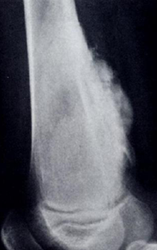
\includegraphics[width=2.70833in,height=2.54167in]{media/image2.png}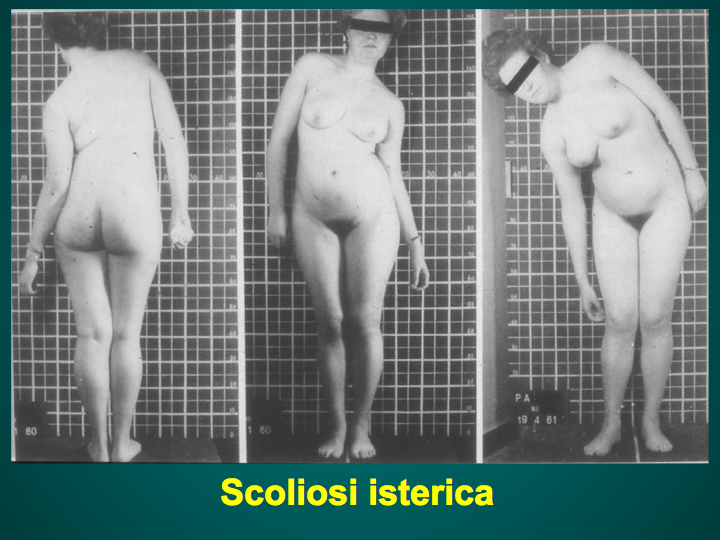
\includegraphics[width=2.51042in,height=2.34375in]{media/image3.png}

\begin{quote}
\textbf{ERNIA CERVICALE}
\end{quote}

Il processo patogenetico prima descritto si traduce in questo segmento
del rachide con una riduzione della fisiologica lordosi, con una
instabilità segmentaria e con la presenza endomidollare o
interforaminale di ernie dure ossia formazioni composte non di nucleo
polposo molle ma da materiale osseo che si crea quando i corpi
vertebrali hanno attrito reciproco -\/-\textgreater{}
\textbf{sindesmofiti e osteofiti interapofisari (ernia dura).}

\begin{quote}
\textbf{Quadri clinici e relative terapie:}
\end{quote}

\begin{itemize}
\item
  \textbf{Cervicalgia}: il dolore è limitato al collo nella sua faccia
  posteriore fino alla nuca ed è esacerbato dalla palpazione dei
  processi trasversi, si associa spesso a vizi posturali che hanno un
  significato antalgico. Il trattamento è sostanzialmente composto da
  FANS , miorilassanti, massoterapia, applicazione locale di calore,
  programma fisioterapeutico.
\item
  \textbf{Cervico-brachialgia:} oltre al dolore al collo c'è un dolore
  irradiato all'arto superiore in quanto il processo degenerativo delle
  articolazione intervertebrali ha portato all'interessamento delle
  radici nervose con conseguente alterazione della sensibilità, della
  forza, e dei riflessi profondi regionali.E' dunque indispensabile
  eseguire un controllo neurologico dell'arto superiore e identificare
  la radice probabilmente coinvolta ricordando che alcuni riflessi
  indagano prevalentemente alcuni mielomeri ( bicipitale = C5,
  brachioradiale = C6 , tricipitale = C7).Il trattamento può avvalersi
  di un uso combinato di cortisonici ad alte dosi per pochi giorni e
  analgesici per controllare la fase irritativa della radiculopatia, si
  può prescrivere pure un collare morbido che applichi una
  decompressione delle radici nervose stesse.Nei casi gravi si può
  ricorrere all'intervento chirurgico decompressivo che, con l'accesso
  chirurgico anteriore o posteriore, permette una discectomia o una
  laminoplastica.
\end{itemize}

\begin{quote}
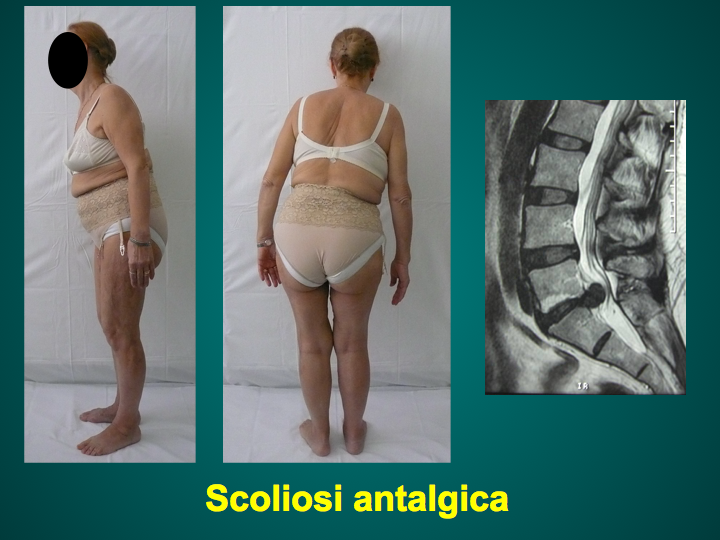
\includegraphics[width=1.92708in,height=2.83264in]{media/image4.png}
\end{quote}

\begin{itemize}
\item
  \textbf{Mielopatia spondilosica e sindromi neuro vascolari:} sono
  quadri molto gravi che necessitano di un rapido inquadramento clinico
  e di un altrettanto rapida soluzione chirurgica. Sono conseguenti alla
  protrusione dentro il canale midollare di un importante volume di
  materia che riesce a comprimere il sacco durale e dunque il midollo e
  i vasi sanguigni corrispondenti. Si presentano con paraparesi
  spastica, iperreflessia e turbe della sensibilità termico dolorifica (
  fascio spinotalamico). Le sindromi neurovascolari sono talvolta
  attribuibili a disordini psicoemotivi del paziente piuttosto che
  all'interessamento dei nervi simpatici; sono invecie frequenti i drops
  attacks riferibili a disordini circolatori nel territorio di
  distribuzione delle arterie vertebrali. La terapia chirurgica è quella
  prima esposta per le forme gravi di cervico-brachialgia.
\end{itemize}

In tutte queste forme la diagnosi si basa sulla clinica e sull'imaging:
radiografie in posizione statica anteroposteriore e latero-laterale, in
massima flessione e in massima estensione per valutare il grado di
instabilità articolare. Per la corretta interpretazione del dolore
neuropatico ci si avvale di indagini neurologiche quali
l'elettromiografia e i potenziali evocati sensitivo-somatici. Tutto
questo vale anche per la prossima sezione.

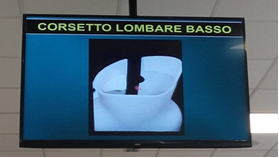
\includegraphics[width=1.50000in,height=2.28125in]{media/image5.png}

\begin{quote}
\textbf{ERNIA LOMBARE}
\end{quote}

In questa sezione del rachide si concentrano due fattori favorenti la
degenerazione discale: l'ampia articolarità e la sopportazione di tutto
il peso del tronco e degli arti superiori.

Molto spesso la sintomatologia è dipendente all'erniazione del nucleo
polposo la quale può essere caratterizzata per tragitto compiuto
(contenuta se il nucleo è rimasto al di sotto del legamento
longitudinale posteriore, espulsa se ha superato il legamento ma ha
mantenuto una continuità con il nucleo discale, migrata se se ne è
completamente distaccata ) o per posizione raggiunta (posteriore,
postero-laterale, intra ed extra foraminale). Ad ogni tipologia di ernia
corrisponde una presentazione clinica conseguente all'interessamento

delle strutture nervose incontrate, il quadro può presentarsi acutamente
o raggiungere l'acme in giorni-settimane.

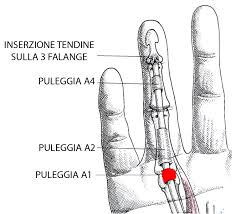
\includegraphics[width=1.15625in,height=1.59375in]{media/image6.png}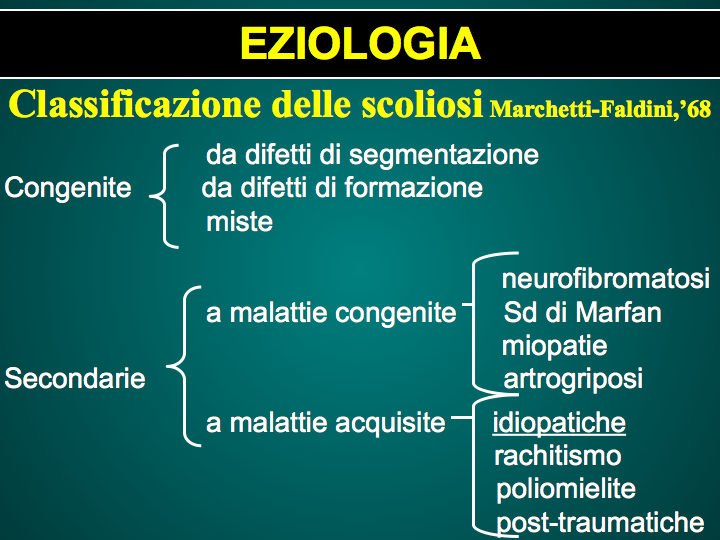
\includegraphics[width=3.29097in,height=2.87431in]{media/image7.png}

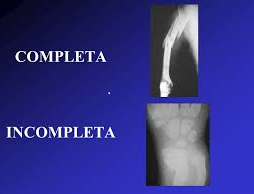
\includegraphics[width=2.03125in,height=1.35417in]{media/image8.png}

\begin{itemize}
\item
  \textbf{Lombocruralgia e lombosciatalgia}: sono caratterizzate da
  dolore in sede lombare con irradiazione o alla faccia anteriore della
  coscia o alla faccia posteriore di tutto l'arto inferiore
  rispettivamente. Come per la cervicobrachialgia è molto importarte per
  fini terapeutici e prognostici caratterizzare il danno neurologico
  conseguente lo schiacciamento radicolare che evolte secondo le tre
  classiche fasi di IRRITAZIONE (clinicamente manifestano dolore),
  DEFICIT (sia il versante motorio che quello sensitivo non sono più
  funzionali e si analizzano investigando la sensibilità
  tattico-termico- dolorifica-pallestesica e la mobilità dei gruppi
  muscolari dei territori innervati da tale radice, si devono inoltre
  investigare i riflessi osteo-tendinei per avere indicazione di sede),
  PARALITICA (completo deficit sensitivo-motorio e atrofia muscolare da
  denervazione + deformità e non funzionalità segmetaria).Clinicamente
  si valutano pure la dolorabilità alla palpazione del decorso dei
  singoli nervi interessati, ossia il femorale per la lombocruralgia e
  lo sciatico-popliteo per la lombosciatalgia, e la dolorabilità evocata
  durante particolari manovre semeiologiche : manovra di Wasserman
  (paziente prono , dolore all'estensione dell'anca con ginocchio flesso
  per stiramento di L4), manovra di Lasegue (paziente supino, dolore
  alla flessione dorsale del piede a ginocchio esteso e anca sollevata a
  45°).La terapia in questi casi si avvale di farmaci analgesici e
  antiinfiammatori non steroidei per i quadri lievi e di cortisonici per
  i quadri deficitari, associati alla prescrizione di un busto
  semirigido che trazioni il rachide e ad un regime di riposo con
  divieto assoluto di sollevare carichi che andrebbero ad aggravare
  l'erniazione del nucleo polposo. I quadri inveterati o particolarmente
  gravi sono indicazioni all'esecuzione di interventi decompressivi
  della cavità midollare o dei forami di coniugazione: discectomia .
  Questi interventi sono gravati da complicazioni serie quali
  l'instabilità del segmento trattato con conseguente lombalgia cronica.
\item
  \textbf{Sciatica paralitica e sindrome della cauda equina}: sono
  quadri molto gravi che si verificano più facilmente in soggetti che
  costituzionalmente hanno già una stenosi del canale vertebrale lombare
  e dunque sono più soggetti allo sviluppo di dolore neuropatico da
  compressione.
\end{itemize}

\begin{quote}
Si caratterizzano per una ipoanesetsia "a sella" che dalla zona
perianale si distribuisce alle zone mediali limitrofe, per turbe
sfinteriche e per paraparesi flaccide. Loro stesse sono indicazioni
all'esecuzione dell'intervento chirurgico che non sempre è risoluitivo.

\textbf{Diagnosi e diagnosi differenziale:}
\end{quote}

le tecniche di imaging risescono a caratterizzare l'enria e a
visualizzare la radice nervosa compressa . Facendo questo riescono ad
escludere altre possibili cause di dolore neuropatico tra le quali:
tumori ossei e nervosi, cisti midollari, tumori retroperitoneali,
malattie infettive.

Particolare attenzione va rivolta a situazioni cliniche che possono
presentarsi con un dolore simile : nefrolitiasi, arteriopatia periferica
con claudicatio intermittens, complicazioni ovarico-annessiali,
coxartrosi e borsiti intertrocanteriche.

\end{document}
